\chapter{Case study 1: Enforcing general best practices}
\label{chap:case_study1}

This chapter showcases the capabilities of the Konstrainer framework through a fictional company's business application. The case study begins by establishing the starting state of a demo application. It then identifies several problems with the application, proposes solutions to those problems, and finally establishes rules that prevent the future occurrence of those problems.

A fictional company, Apples Inc., embarked on a journey to modernize its business operations. The mangers decided that buying an existing solution is too expensive, so they opted for a custom application built by their engineers. They specifically mandated that the application be built upon the microservices architecture and run in Kubernetes, mainly because this is trendy today, even thought they did not properly investigate whether it is the best solution for their use-case or not. Moreover, the engineers lacked prior experience with Kubernetes. The combination of insufficient experience, inadequate planning, and tight deadlines led to numerous mistakes in the development process.

Their application is still a work in progress, with limited functionality - it serves as a small demo solely for the purpose of this case study.

\section{Setup}

I have prepared this demo on GitHub: \url{https://github.com/Tiegris/KonstrainR/tree/main/main/DemoApp}

The repository is publicly available, enabling readers to download it, try it out, and follow along with this demonstration. If you do not wish to check out the repository, the referenced resource files can also be found in the appendix.

Requirements:

\begin{itemize}
    \item Docker
    \item Playground Kubernetes cluster (Tested with version: v1.27.2)
    \item Helm
    \item yq (Tested with version: (\url{github.com/mikefarah/yq/}) version 4.18.)
\end{itemize}

The demo was tested on Ubuntu 22 with bash.

If you follow along, make sure that you are in the \emph{main/DemoApp} folder of the repository.

Execute the initial setup script: \lstinline|./initial-setup.sh| This script establishes the initial state of the demo system by replicating commands that the developers of the system might have used, or running commands that simulate steps of the development process.

\subsection{Breakdown of setup}

This section breaks down the steps of the setup script and explains each step, by telling a story what the developers did, to achieve the current state of the system.

When the initial two microservices for the app were developed, the developers created a YAML file for each and defined the essential Kubernetes resources required for them:

\begin{lstlisting}[caption={Create first deployment},language=bash,label=code:bash3]
# Initial creation of users app
kubectl create ns users
kubectl apply -n users -f $home/k8s/users.yaml

# Initial creation of items app
kubectl create ns items
kubectl apply -n items -f $home/k8s/items.yaml
\end{lstlisting}

The resource descriptions were generated using the VS Code Kubernetes extension\footnote{\url{https://github.com/vscode-kubernetes-tools/vscode-kubernetes-tools}} and slightly customized, so most values were left on default.

Note that the items.yaml (\ref{appendix:csr:items}) contains an unused \emph{PersistentVolumeClaim} (PVC). This could be the result of a copy and paste oversight, or just someone forgot to delete it. We will use Konstrainer to detect it.

The `items' app went through a long development. The setup script simulates the multiple redeployment of the app, as shown in the \ref{code:bash4} snippet.

\begin{lstlisting}[caption={Simulate redeployment of the `items' app},language=bash,label=code:bash4]
# Simulate a history of changes
for v in {1..14}; do
    yq eval 'select(.kind == "Deployment").spec.template.metadata.annotations.v = env(v)' $home/k8s/items.yaml -i
    kubectl apply -n items -f $home/k8s/items.yaml
done
# Restore yaml file
yq eval 'select(.kind == "Deployment").spec.template.metadata.annotations.v = "0"' $home/k8s/items.yaml -i
\end{lstlisting}

The engineers in charge of the Kubernetes deployments set up test environments for experimentation and testing purposes, but they neglected to delete them. This is simulated by the \ref{code:bash5} code snippet.

\begin{lstlisting}[caption={Simulate leftover resources},language=bash,label=code:bash5]
  # Simulate John Athan creating test namespace
  kubectl create ns jathan-test || true
  # Simulate Ida Red creating test namespace and leaving some leftover resources in it
  kubectl create ns ired-test || true
  kubectl apply -n ired-test -f $home/k8s/junk.yaml
\end{lstlisting}

The developers decided that they want to use a NoSQL database. They searched the internet, and one of the first search results was this: \url{bitnami.com/stack/mongodb/helm}. This website shows a command that looks like it deploys a MongoDB. The engineers tested it, and it worked. They did not bother with reading the documentation or properly configuring the database; there was no time for that. The \ref{code:bash5b} snippet shows how they used the code from the website.

\begin{lstlisting}[caption={Deploy MongoDB},language=bash,label=code:bash5b]
kubectl create ns mongo
helm install -n mongo my-release \
  oci://registry-1.docker.io/bitnamicharts/mongodb
\end{lstlisting}

After deploying MongoDB, the engineers configured the `items' service to use it. They manually edited the items.yaml file and changed the code based on the first tutorial they could find. The image used by the `items' deployment already uses MongoDB; the commands in the \ref{code:bash7} code snippet only emulate this process.

\begin{lstlisting}[caption={Configuring the `items' app to use MongoDB},language=bash,label=code:bash7]
export MONGODB_ROOT_PASSWORD=$(kubectl get secret --namespace mongo \
  my-release-mongodb -o jsonpath="{.data.mongodb-root-password}" \
  | base64 -d)
export MONGO_HOST="my-release-mongodb.mongo.svc.cluster.local"
yq eval 'select(.kind == "Deployment").spec.template.spec.containers[0].env[0].value = env(MONGODB_ROOT_PASSWORD)' $home/k8s/items.yaml -i
yq eval 'select(.kind == "Deployment").spec.template.spec.containers[0].env[1].value = env(MONGO_HOST)' $home/k8s/items.yaml -i
kubectl apply -n items -f $home/k8s/items.yaml
\end{lstlisting}

At this point, we have a demo application running which resembles a system with many mistakes.

\subsection{Test and teardown the demo application}

If you have followed along, make sure to test the deployment. First check the status of all \emph{Pod}s, by executing: \lstinline|kubectl get pods -A| All the \emph{Pod}s should have the status: `Running', except the `my-test-2' \emph{Pod}.

You can also test the integration of the items app and the MongoDB by executing the commands in the \ref{code:bash8} snippet.

\begin{lstlisting}[caption={Test the integration of the items app and MongoDB},language=bash,label=code:bash8]
kubectl port-forward -n items service/items 8080:8080
# In a separate terminal
curl http://localhost:8080/items
# You should get a valid JSON as result
\end{lstlisting}

If you wish to uninstall the demo and the Konstrainer application run the code in the \ref{code:bash9} snippet.

\begin{lstlisting}[caption={Teardown},language=bash,label=code:bash9]
# Uninstall demo app
helm uninstall my-release -n mongo
kubectl delete ns users items jathan-test ired-test mongo
# Uninstall Konstrainer
helm uninstall konstrainr-core -n konstrainer-ns
kubectl delete ns konstrainer-ns
\end{lstlisting}

\section{Introduce policies}

To follow along, you can install the Konstrainer application using a helm chart, as shown in the \ref{code:bashk1} code snippet.

\begin{lstlisting}[caption={Install Konstrainer},language=bash,label=code:bashk1]
cd ../charts
kubectl create ns konstrainer-ns
helm upgrade konstrainr-core konstrainr-core -n konstrainer-ns --install
\end{lstlisting}

Wait for it to start, then port forward the core component: \lstinline|kubectl port-forward service/konstrainer-core 8443:8080 -n konstrainer-ns|
This will allow you to access its frontend in your browser.

\subsection{Basic Diagnostics}

I have collected a set of best practices, and implemented them in my DSL. I implemented them in two files, the first file contains a script which creates a diagnostics report on the cluster including potential bugs and bad practices. This is the \emph{basic diagnostic} script, which can be found in the project repository at the \url{$PROJECT_ROOT/main/Konstrainer-Dsl/src/main/kotlin/me/btieger/builtins/} folder.

If you visit \url{https://localhost:8443}, and configure your browser to trust the self-signed certificate you should see the Web UI. For login, use \emph{admin:admin}. 

After uploading the \emph{basic diagnostic} script, we will see something like in the \ref{fig:case_1} image.

\begin{figure}[h]
  \centering
  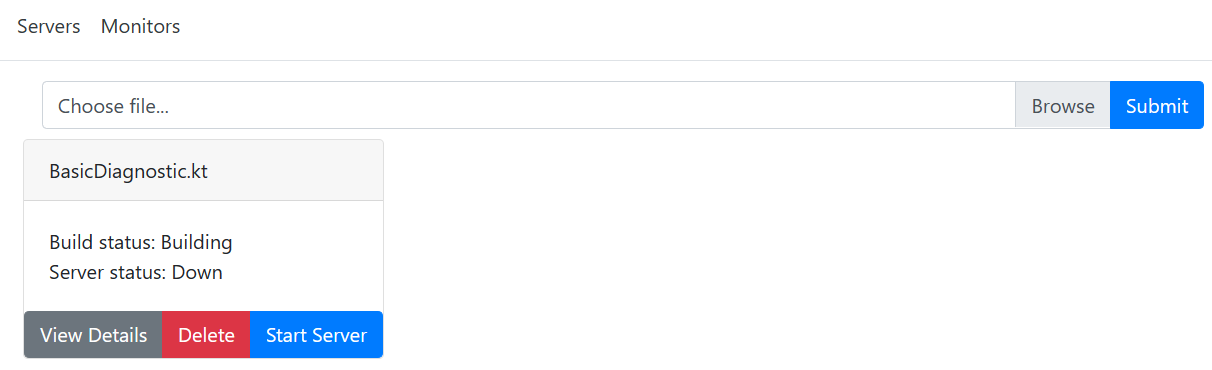
\includegraphics[width=130mm, keepaspectratio]{content/30_caseStudy1/main_menu_with_uploaded_building_dagnotics.png}
  \caption{Konstrainer Web UI with uploaded basic diagnostics script}
  \label{fig:case_1}
\end{figure}

The Web UI had a low priority when creating the project, so the site does not refresh automatically, refresh the page after about 20 seconds to see if it's compiled. You should see: `Build status: Ready'

Click `Start Server'. Wait for it to start. After about 5 seconds refresh the page. You should see: `Server status: Up'

Click `Monitors' in the navigation menu. You should see the report generated by the DSL script. I also included the generated report in this document as in an image, referenced by \ref{fig:case_2}. Note that if you have followed along, your report will look slightly different, because I had to edit the picture to fit into the document.

\begin{figure}[h]
  \centering
  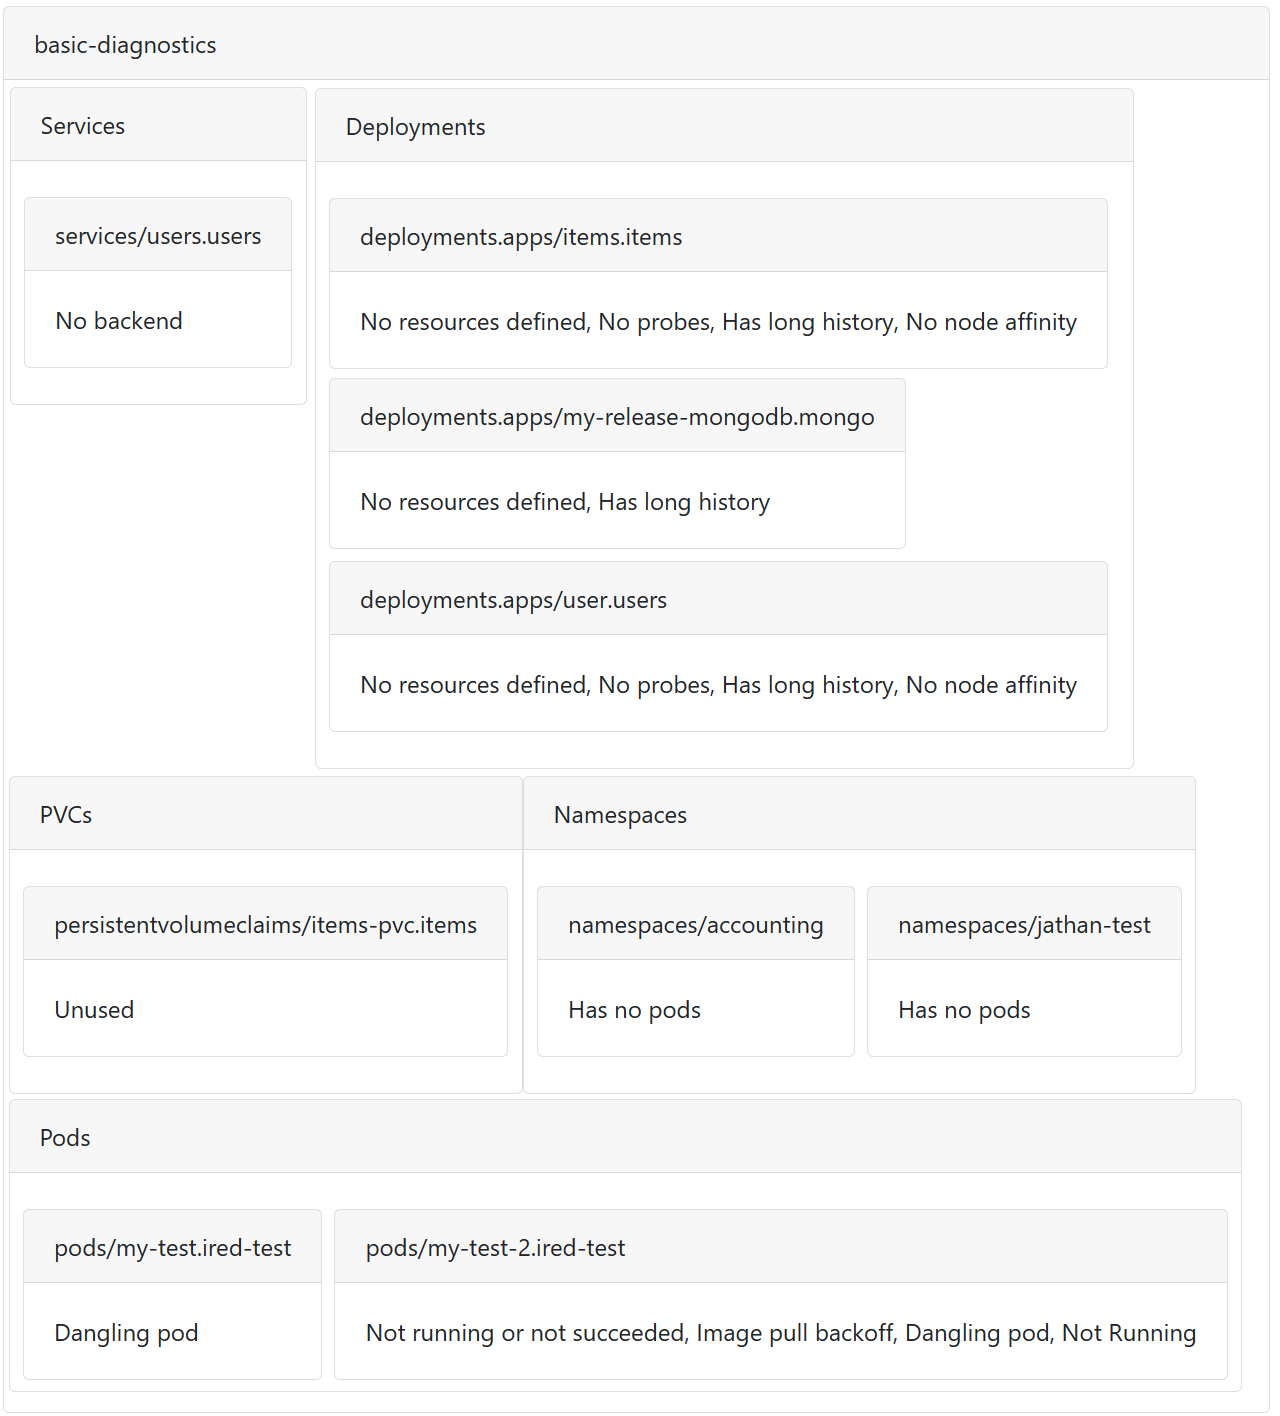
\includegraphics[width=150mm, keepaspectratio]{content/30_caseStudy1/report.png}
  \caption{Basic diagnostics report}
  \label{fig:case_2}
\end{figure}

Let's inspect the report, read it as described below:

The outermost box is an agent, which is a web server, serving the compiled script. It contains many aggregation groups. An aggregation group is a bundle of problems, warnings or policy violations usually about the same kind of Kubernetes resources. The first aggregation group in this report is the: `Services'

Inside an aggregation group there are Kubernetes resources listed which are tagged. In the `Services' aggregation group the only tagged resource is the: `services/users.users'. The format of the tagged Kubernetes resources are: `apiKind/name.namespace'

Under the names of each tagged resource, there is the list of tags. In this case the only tag is: `No backend', which means that the service has no \emph{Pod}s at all, not even unhealthy ones.

Let's find the cause of the problem. The users service was deployed during the initial-setup, using the users.yaml\ref{appendix:csr:users} file. If we inspect this file very carefully, we can see that the selector of the service is looking for pods with the labels: `app: users', but the deployment defines pods with the label: `app: user`. To be honest, this is a very easy typo to make, so in this case we discovered a bug with Konstrainer.

The next aggregation group is the `Deployments'. The most common tags are:

\begin{itemize}
  \item \textbf{No resources defined:} This means that not all containers in the pods of the deployment have resource requests or limits set. While it is a warning, it is usually considered good practice to set these values
  \item \textbf{No node selector:} This means that there is no logic provided on which node (usually a virtual machine) should the pods of the deployment run.
  \item \textbf{No probes:} No liveness probes are defined. Without probes, the Kubernetes API cannot determine if a pod is healthy or not, so it is considered good practice to define probes.
  \item \textbf{Has long history:} The revisionHistoryLimit of the deployment is set to more than 4. The revisionHistoryLimit determines how many replicasets the deployment should keep as a history. The default is 10, but setting it too high can result in a lot of unused resources, putting unnecessary load on the Kubernetes API. It is considered a good practice to set it a low number. This practice was even more crucial in the past when deployments had no default revisionHistoryLimit. According to a blog post~\cite{RevisionHystory}, unused replicasets can cause up to a 10\% unnecessary CPU load clusterwide.
\end{itemize}

The subsequent aggregation group is the `PVCs'. It indicates that there is a \emph{PersistentVolumeClaim}, specifically named `items-pvc', which is unused. Upon inspecting the items.yaml file (\ref{appendix:csr:items}), it becomes apparent that this PVC is not utilized and may be the result of a copy-paste error or a leftover artifact from the project's evolution. Dangling PVCs can incur costs, as although storage is generally inexpensive, if numerous PVCs claim storage from a cloud provider and remain unused, the cumulative cost can escalate quickly. 

The following aggregation group is the `Namespaces'. It indicates that the `jathan-test' namespace has no pods. It is a common practice for developers to create a test namespace as a sandbox for their work. However, it's equally common for these namespaces to be left behind when the work is finished, and developers may forget to delete them. In our case, it appears that the engineer John Athan might have overlooked removing his playground namespace.

The last aggregation group is the `Pods', with two items. The first is the `my-test' pod in the `ired-test' namespace. It is a dangling pod, which means that there is no operator resource (e.g.: a deployment or statefulset) managing its lifecycle. The seconds pod, `my-test-2', presents more problems; it is not running because the Docker image of the pod could not be pulled.  In both cases, these pods were likely created by a developer for testing or development purposes, but were forgotten and not deleted.

This concludes the report created by my script. Issues like this can occur in real life scenarios, and fixing them can improve reliability, performance, maintainability, and cut costs.

\subsection{Introducing basic rule enforcement}

The second script I prepared for the case study does not create a report, but rather enforces best practices by intercepting requests to the Kubernetes API.
This file describes basic rules that are evaluated upon events, like deployment creation. This can be used to prevent the creation of poorly configured resources, and can enforce best practices from the beginning.

To follow along, upload the \emph{basic enforce} script located in the same directory as the \emph{basic diagnostics} script.

Let's deploy the new component of Apples Inc.'s application. First, let's create a namespace like showed in the \ref{code:basha1}

\begin{lstlisting}[caption={Create namespace for the Accounting module},language=bash,label=code:basha1]
cd DemoApp
kubectl apply -f - <<EOF
apiVersion: v1
kind: Namespace
metadata:
  name: accounting
  labels:
    managed: "true"
EOF
\end{lstlisting}

Note that the namespace has a label: `managed: "true"'. This is because my script is configured to only intercept events in the those namespaces, where this label is set.

Now if we deploy the new component, but we forget to switch to the newly created namespace (run code: \ref{code:basha2}) we get a warning: `Warning: You are working in the namespace: default`

\begin{lstlisting}[caption={Deploy the Accounting module},language=bash,label=code:basha2]
# Make sure that you are in the default namespace
kubectl config set-context --current --namespace=default
kubectl apply -f k8s/accounting.yaml
\end{lstlisting}

If you work in the default namespace that might be a mistake, so my Konstrainer script warns you. Let's revert with this command: \lstinline|kubectl delete deployment.apps/accounting| and use the correct namespace from now on.

\begin{lstlisting}[caption={Delete Accounting module from the default namespace},language=bash,label=code:basha3]
kubectl delete deployment.apps/accounting

\end{lstlisting}

If we retry in the correct namespace with the \lstinline|kubectl apply -f k8s/accounting.yaml --namespace=accounting| command, we will get the following error: `Error from server: error when creating "k8s/accounting.yaml": admission webhook "node-affinity.btieger.me" denied the request: Deployment must have some kind of node affinity! (affinity, nodeSelector, nodeName)'

It is generally a good practice to define some kind of logic on how to place our pods. There can be many principals, this rule only requires to define something. In a real scenario we should define at least a nodeSelector, but for now let's just set the nodeName field.

Let's fix this error with the help of the \ref{code:basha5} code snippet. Depending on your cluster chose a suitable node from the output of the get nodes command.

\begin{lstlisting}[caption={Fix node affinity error},language=bash,label=code:basha5]
# This will list all nodes
kubectl get nodes -A
# chose one, eg.:
export node_name="docker-desktop"
yq eval 'select(.kind == "Deployment").spec.template.spec.nodeName = env(node_name)' k8s/accounting.yaml -i
kubectl apply -f k8s/accounting.yaml --namespace=accounting
\end{lstlisting}

Now that we've addressed the node affinity problem, upon retrying, we encounter another issue: `Error from server: error when creating "k8s/accounting.yaml": admission webhook "deny-no-resources.btieger.me" denied the request: Deployment must have resource definitions!'

Setting resource limits and requests is a standard practice. In short, a cluster can work just fine without them, but neglecting them can result in stability issues~\cite{ResourcesGood}. For a more in-depth explanation, I recommend reading the cited source.

In a real-world scenario, to determine the correct resource settings, we should first make an estimate and refine it with measurements. Since this is just a demo, setting an estimate is fine. The \ref{code:basha7} shows how to set them.

\begin{lstlisting}[caption={Setting resources and redeploy the Accounting module},language=bash,label=code:basha7]
yq eval 'select(.kind == "Deployment").spec.template.spec.containers[0].resources.limits.cpu = "500m"' k8s/accounting.yaml -i
yq eval 'select(.kind == "Deployment").spec.template.spec.containers[0].resources.limits.memory = "128Mi"' k8s/accounting.yaml -i
yq eval 'select(.kind == "Deployment").spec.template.spec.containers[0].resources.requests.cpu = "500m"' k8s/accounting.yaml -i
yq eval 'select(.kind == "Deployment").spec.template.spec.containers[0].resources.requests.memory = "128Mi"' k8s/accounting.yaml -i
kubectl apply -f k8s/accounting.yaml --namespace=accounting
\end{lstlisting}

This time the deployment succeeded, but we got some warnings:

\begin{itemize}
  \item Warning: No security context
  \item Warning: RevisionHistoryLimit was set to 4, from original: 10
\end{itemize}

The first warning indicates that we have not yet defined a security context, while the second tells us that the revisionHistoryLimit of the deployment was changed. Konstrainer allows creating rules that not only reject some actions but also perform minor alterations.

Upon inspecting the newly created deployment, we can observe that the revisionHistoryLimit has indeed been modified:
\lstinline|kubectl get deployment accounting -n accounting -o yaml | yq '.spec.revisionHistoryLimit'|

In this chapter, I presented the motivation behind the Konstrainer project by highlighting some common and easily overlooked mistakes. Following that, I demonstrated the power of the Konstrainer platform and showcased the capabilities of my pre-made scripts for enforcing best practices. 

The next chapter interrupts the case study to provide a detailed explanation of my DSL. Understanding the core concepts and language features is crucial for the upcoming sections of the case study, which will be continued in Chapter \ref{chap:case_study2}~\nameref{chap:case_study2}.

TODO put scripts in appendix

